%!TEX root = ../main.tex
% !TeX encoding = UTF-8
\section{Experimentos}

    \subsection{Capacete para Segurança de Ciclistas}
        Desenvolveu-se um protótipo de capacete na qual realiza-se verificações de distância de objetos nas costas do ciclista a fim de alertá-lo de possíveis riscos de acidentes.
        Caso esteja em situação de risco, o capacete emitirá sinais visuais luminosos, além do envio de aviso para um segundo dispositivo avisando de sua situação sendo este não fazendo parte do trabalho.
        Para dados mais coerentes com a distância real, construiu-se um capacete modular a fim de fazer diferentes testes sendo então, com 1 à 3 sensores de distância além de um \buffer\ de dados de tamanho 5, 10 e 15 para processamento das distâncias de cada sensor, discutidos a seguir.
        
        \begin{figure}[h] \centering
            \vspace{-0.5em}
            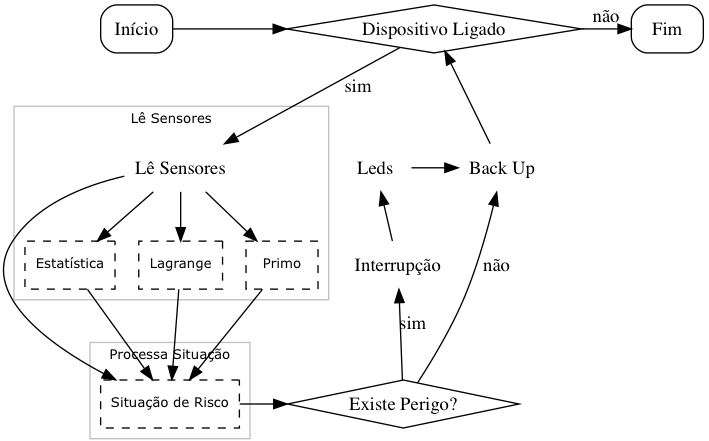
\includegraphics[width=0.48\textwidth]{img/capacete.png}
            \caption{Grafo de chamada do algoritmo base do \wearable.}
            \label{fig:gc}
        \end{figure}
        
        Como é exibido na Figura \ref{fig:gc}, os passos do \wearable\ constituem-se basicamente de leitura das distâncias, cálculo de risco e aviso ao usuário.
        O particionamento será avaliado em duas seções principais, sendo elas a de leitura e de processo de situações, constituindo de 4 situações diferentes de particionamento para análise.
        Na seção de leitura de sensores, serão adicionados: \textit{1)} algoritmo de análise estatística (Algoritmo \ref{alg:statistic}) na qual calculará valores de desvio padrão e variância dos valores no \buffer; \textit{2)} algoritmo de lagrange (Algoritmo \ref{alg:lagrange}) interpolará novas distâncias e; \textit{3)} algoritmo de números primos (Algoritmo \ref{alg:prime}) avaliará se a soma das distâncias lidas correspondem à números primos.
        A análise serão feitas por meio de exclusão, selecionando apenas um algoritmo por vez e adicionado ao código para análise.
        Quando nenhum desta seção for utilizado para particionamento, utiliza-se então: \textit{4)} algoritmo de processamento de risco (Algoritmo \ref{alg:risk}), na seção de processo de situações.
        Este por sua vez está em todas as análises, pois é passo necessário para a iteração do \wearable.
        
    
        A placa utilizada para sintetização foi uma Arty A7-35T.% com 32 mil elementos lógicos e \textit{clock} de 450MHz.
        Utilizou-se o sistema \textit{soft-processor} MicroBlaze para processamento do código em \software.
        Todos os algoritmos foram construídos utilizando ferramenta HLS \todo{sigla} e incorporados ao projeto base.
        A comunicação entre \hs\ é feita utilizando interface AXI.
        A medição de distância é realizada com um sensor ultrassônico e a comunicação com o segundo dispositivo utiliza \textit{Bluetooth Low Energy}.
        
        
    \subsection{Testes Realizados}
        % Explicando os testes
        Para a realização dos testes, será feito um procedimento tendo base a Figura \ref{fig:distance}. 
        O teste possui 2 passos, a aproximação e o distanciamento de objeto, na qual serão aplicados no decorrer de 12 iterações do \wearable.
        %
        \textit{Iteração 1:} o ciclista encontra-se a uma distância de 130 centímetros do objeto, sendo sua situação declarada como Segura;
        %
        \textit{Iteração 4:} o objeto inicia um movimento de aproximação ao ciclista chegando a ultrapassar o limite mínimo de 30 centímetros iniciando a situação de Risco;
        %
        \textit{Iteração 9:} o objeto afasta novamente do ciclista para 130 centímetros, retornando à situação Segura.
        Tanto o movimento de aproximação quanto o de afastamento são feitos manualmente para que simule de fato a situação real de um ciclista em seu meio;
        \textit{Iteração 12:} última leitura para testes.
        %
        Sendo assim, cada algoritmo será performa e separadamente analisados em ambos os níveis de \software\ e \hardware.
        Para uma análise estatística dos resultados, esse conjunto de 12 iterações e os respectivos movimentos repetirão por 30 vezes.

        \begin{figure}[h] \centering
            \vspace{-1em}
            
\includegraphics[width=0.5\textwidth]{img/distance.png}
            \caption{Testes de resposta do \wearable\ à situações de possível perigo.}
            \label{fig:distance}
        \end{figure}

\section{Resultados}
    % tabela hls
    Os recursos utilizados em cada algoritmo ao realizar o seu particionamento é exibido na Tabela \ref{tab:hls}.
    \begin{table}[h]\centering
        \vspace{-1em}
        \scriptsize
        %\raaa{1.0}
        \raaa{0.9}
        \caption{Recursos Utilizados no HLS.}
        \begin{tabular}{rrr|rr|rr|rr||rr}
            \toprule
            &\multicolumn{2}{c}{Expressões} & \multicolumn{2}{c}{Instâncias}      & \multicolumn{2}{c}{Multiplex}  & \multicolumn{2}{c}{Regist.} & \multicolumn{2}{c}{\textit{Total}} \\
            \cmidrule{2-11}
            %\cmidrule{2-3} \cmidrule{5-6} \cmidrule{8-9} \cmidrule{11-12} \cmidrule{14-15}
            & \textit{Lut} & \textit{Ff} & \textit{Lut} & \textit{Ff} & \textit{Lut} & \textit{Ff} & \textit{Lut} & \textit{Ff} & \textit{Lut} & \textit{Ff} \\
            \midrule
            \A$_1$&52 & 0     & 1948 & 1474   & 364 & 0      & 0 & 394   & 2364 & 1868 \\ 
            \A$_2$&128 & 0    & 2048 & 1425   & 309 & 0      & 0 & 479   & 2483 & 1904 \\ 
            \A$_3$&1826 & 0   & 486 & 552     & 236 & 0      & 0 & 527   & 2448 & 1079 \\ 
            \A$_4$&18 & 0     & 120  & 82     & 15  & 0      & 0 & 34    & 153  & 116  \\ 
            \bottomrule
        \end{tabular}
        \label{tab:hls}
    \end{table}

    % tabela vivado
    Ao adicionar o algoritmo em \hardware\ ao projeto base é possível calcular seu gasto de recursos bem como seu gasto energético.
    Tais valores são exibidos na Tablea \ref{tab:vivado}.
    \todo[inline]{parei aqui}
    \begin{table}[h]\centering
        \vspace{-1em}
        \scriptsize
        %\raaa{1.0}
        \raaa{0.9}
        \caption{Recursos Utilizados no Projeto Final.}
        \begin{tabular}{rcccccc}
            \toprule
            %&\multicolumn{2}{c}{Expressões} & \multicolumn{2}{c}{Instâncias}      & \multicolumn{2}{c}{Multiplex}  & \multicolumn{2}{c}{Regist.} & \multicolumn{2}{c}{\textit{Total}} \\
            %\cmidrule{2-11}
            %\cmidrule{2-3} \cmidrule{5-6} \cmidrule{8-9} \cmidrule{11-12} \cmidrule{14-15}
            & LUT    & LUTRAM   & FF     & I/O     & On-Chip Power & Off-ChipPower \\
            \cmidrule{2-7}
            
                  & 20800  & 9600     & 41600  & 210    & -              & -      \\
            \A$_1$& 13640  & 1822     & 13080  & 104    & 0,972W         & 0,506W \\ 
            \A$_2$& 13502  & 1808     & 13193  & 104    & 0,968W         & 0,506W \\ 
            \A$_3$& 12959  & 1782     & 12559  & 104    & 0,933W         & 0,506W \\
            \A$_4$& 12109  & 1781     & 11742  & 104    & 0,929W         & 0,506W \\ 
            \bottomrule
        \end{tabular}
        \label{tab:vivado}
    \end{table}

    %tabela ms
    A Tabela~\ref{tab:iterations} exibe os valores obtidos da análise de performance comparando os sistemas em \software\ e \hardware. 
    Valores exibidos mostram a diferença performática de \software\ e \hardware\ sendo que os valores positivos indicam o tempo na qual o algoritmo \A$_i$ obteve maior performance em \hardware, enquanto valores negativos exibem maior performance em \software, todos em milissegundos.
    As informações exibidas foram filtradas, eliminando o tempo médio gasto da atuação dos sensores bem como o tempo de envio para o dispositivo externo, ambos dependente de sua tecnologia.

    \begin{table}[h]\centering
        \vspace{-1em}
        \scriptsize
        %\raaa{1.0}
        \raaa{0.9}
        \caption{Recursos Utilizados no HLS.}
        \begin{tabular}{@{}crrr|rrr|rrr@{}}\toprule
            & \multicolumn{3}{c}{1 Sensor} & \multicolumn{3}{c}{2 Sensores} & \multicolumn{3}{c}{3 Sensores}\\
            \cmidrule{2-10}
            %\cmidrule{2-4} \cmidrule{6-8} \cmidrule{10-12} \textit{} 
            & \textit{b}:\,5 & \textit{b}:\,10 & \textit{b}:\,15 & \textit{b}:\,5 & \textit{b}:\,10 & \textit{b}:\,15 & \textit{b}:\,5 & \textit{b}:\,10 & \textit{b}:\,15 \\
            \midrule
            %\textit{sistêmica} \\
            %média     & ? & ? & ? & ? & ? & ? & ? & ? & ? \\
            \A$_1$   & -2.0   &    0.5  &    0.4  &   -2.7  &   -1.6  &   -1.8  &    0.4  &   0.3   &     4.2   \\
            \A$_2$   &  7.7   &    9.3  &    8.6  &   10.9  &    9.9  &   11.6  &   10.2  &   12.0  &    12.1   \\
            \A$_3$   &  2.8   &   12.2  &   91.8  &    1.6  &   44.6  &   13.9  &    4.1  &   64.8  &   231.3   \\
            \A$_4$   & 17.8   &   17.2  &   16.9  &   15.0  &   14.9  &   12.9  &   15.0  &   17.5  &    18.4   \\
            \bottomrule
        \end{tabular}
        \label{tab:iterations}
    \end{table}

    Os algoritmos \A$_i$ representam respectivamente Estatístico, Lagrange, Números primos e Risco, variando o número de sensores e o tamanho de seu \buffer\ interno.
  

\begin{comment}
    Expression & Instance      & Multiplexer  & Register & Total
    52 / 0     & 1948 / 1474   & 364 / 0      & 0 / 394   & 2364 / 1868 \\ statistic
    128 / 0    & 2048 / 1425   & 309 / 0      & 0 / 479   & 2483 / 1904 \\ lagrange
    1826 / 0   & 486 / 552     & 236 / 0      & 0 / 527   & 2448 / 1079 \\ prime
    18 / 0     & 120  / 82     & 15  / 0      & 0 / 34    & 153  / 116  \\ risk
    
    
    & LUT    & LUTRAM   & FF     & IO     & On-Chip Power & Power supplied to off-chip devices
    & 20800  & 9600     & 41600  & 210    & -             & - \\
    & 13640  & 1822     & 13080  & 104    & 0,972         & 0,506 \\ statistic
    & 13502  & 1808     & 13193  & 104    & 0,968         & 0,506 \\ lagrange
    & 12959  & 1782     & 12559  & 104    & 0,933         & 0,506 \\ prime
    & 12109  & 1781     & 11742  & 104    & 0,929         & 0,506 \\ risk
    
\end{comment}


\begin{comment}
    \begin{table}\centering
    \scriptsize
    \raaa{1.3}
    \caption{Cálculo de performance sobre variações em I/O e algoritmo particionado.}
    \begin{tabular}{@{}rrrrcrrrcrrr@{}}\toprule
    & \multicolumn{3}{c}{$\mathcal{O}(1)$} && \multicolumn{3}{c}{$\mathcal{O}(n)$} & & \multicolumn{3}{c}{$\mathcal{O}(n\log n)$}\\
    \cmidrule{2-4} \cmidrule{6-8} \cmidrule{10-12}análise& 5 & 10 & 15 && 5 & 10 & 15 &&5 & 10 & 15 \\
    \midrule \textit{sistêmica} \\
    %média     & ? & ? & ? && ? & ? & ? && ? & ? & ? \\
    $\bar{x}$     & ? & ? & ? && ? & ? & ? && ? & ? & ? \\
    $\sigma^2$ & ? & ? & ? && ? & ? & ? && ? & ? & ? \\
    $\sigma$ & ? & ? & ? && ? & ? & ? && ? & ? & ? \\
    \midrule \textit{empírica} \\
    %média     & ? & ? & ? && ? & ? & ? && ? & ? & ? \\
    $\bar{x}$     & ? & ? & ? && ? & ? & ? && ? & ? & ? \\
    $\sigma^2$ & ? & ? & ? && ? & ? & ? && ? & ? & ? \\
    $\sigma$ & ? & ? & ? && ? & ? & ? && ? & ? & ? \\
    \bottomrule
    \end{tabular}
    \end{table}
    \end{frame}
\end{comment}

